\section{Painting Detection}
\label{sec:painting_detection}




	The core of this work is painting detection, which consists of two steps: painting segmentation and feature matching. The segmentation tries to extract paintings from an arbitrary image while feature matching attempts to find distinguishable features of the extracted paintings and to match it against a database of paintings.

	\subsection{Painting Segmentation}
	The first step of the algorithm is the segmentation of an arbitrary video frame to detect a painting. A typical painting contains the art on its own enclosed by a painting frame. This painting frame causes a strong change in environment around its edges. For that reason, the Canny operator is applied to the initial video frame, resulting in a new image which contains strong edges. Afterwards, we attempt to find contours which yields a vector of points for each contour. To make this process easier and more accurate, a dilation step is first applied on the edge image. We consider only contours which consists of 4 points and take the first 10 which have the highest area, as paintings tend to have a higher area than other quadrilaterals on a video frame. It is possible that multiple paintings exist on a single video frame. However, the algorithm's goal is to detect in which room the user is located, and not in particular which painting it is. Multiple paintings on the same wall belong to the same room. If the painting segmentation step selects either one of these paintings, the end result will be the same. 
	

	The detected painting is then transformed through a homography to a rectified version which serves as the input of the following stage, feature detection and matching.

	\subsection{Feature Detection and Matching}
	Feature detection and extraction is applied to the extracted painting from the segmentation phase and will be matched with an image from the database. The detection of key features and descriptors is handled by ORB. Matching is done by invoking a matching procedure between the extracted keypoints and the keypoints of the database images. A match between descriptors is defined by its distance metric. The lower this number, the more likely that the match is valid. We calculate the sum of all matches and sort the matches between the source and database images by this sum. The first entry in this collection of matches is the image that is estimated to be a match for what is currently seen on-screen. 

	Additional meta-data is associated with the matched image and is used for the next phase.

	\subsection{Path Tracking}
	Once a painting is identified and matched, it can be localized on the ground plan. To achieve this, the ground plan is converted into a directed graph. The nodes of this graph are the rooms of the museum and the edges define the connections between rooms. When a painting is matched, its room is also known. This room can be marked on the graph in three distinct ways. A green node is the start of the path, an orange node is an intermediate path and the blue node is the end of the path. The path ends when the runtime loop ends. The path direction is also visualized by coloring the corresponding edges green. Note that when a cyclic path occurs which was walked in both directions, information of order of the nodes in this cycle is lost.


	To illustrate the path tracking algorithm,  a small segment consisting of rooms 1, 2, 3, 4, 5, 6, 7 and 8 are converted into such a graph and are show on figure \ref{fig:groundplan_msk_simple_graph}.


	%digraph G {
	%	2[fontcolor=white, fillcolor=green, style=filled]	
	%	4[fillcolor=orange, style=filled]
	%	5[fillcolor=orange, style=filled]
	%	7[fillcolor=orange, style=filled]
	%	6[fontcolor=white,fillcolor=blue, style=filled]
	%	1 -> 2
	%	2 -> 1
	%	2 -> 3
	%	2 -> 4[color=green]
	%	2 -> 5
	%	3 -> 2
	%	4 -> 2
	%	4 -> 5[color=green]
	%	4 -> 7
	%	4 -> 8
	%	5 -> 7[color=green]
	%	7 -> 6[color=green]
	%	6 -> 7
	%	7 -> 8
	%	7 -> 5
	%	7 -> 4
	%}

	\begin{figure}
		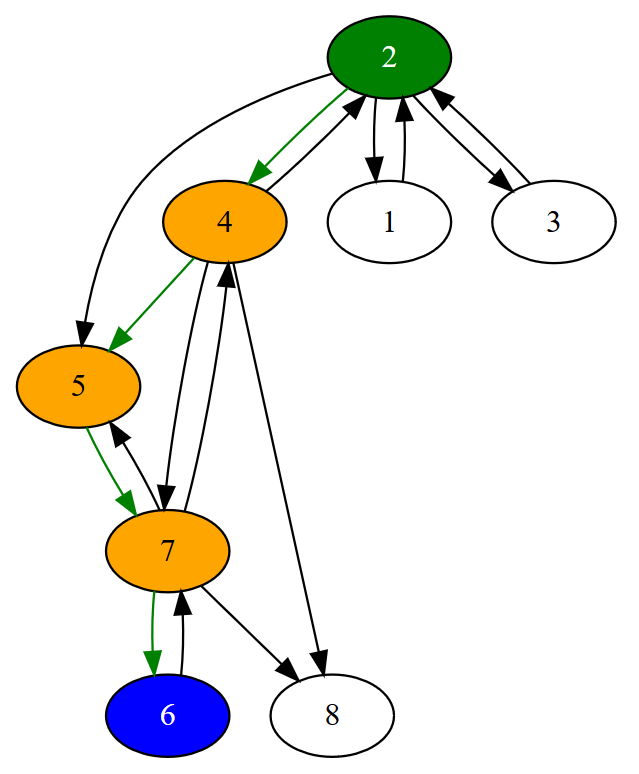
\includegraphics[width=\linewidth]{groundplan_msk_simple_graph}
		\caption{Path tracking using a graph. A green node marks the path's start, orange nodes the visited rooms, and blue the last node that was visited. Edges in green help visualize the path and the order which it was travelled.}
		\label{fig:groundplan_msk_simple_graph}
	\end{figure}

